\section{Methodology}\label{sec:meth}

Our methodology consists of two main phases. In the first phase, we replicate the synthetic market environment developed by \textcite{fish_algorithmic_2025}, using it as a testbed to evaluate the behavior of various open-source LLMs as pricing agents. While the environment itself remains unchanged, our contribution lies in replacing the proprietary LLMs used by the authors with open-source alternatives and extending the analysis beyond monopoly and duopoly to an oligopoly setting. \textcolor{red}{Furthermore, we introduce cost shocks in the environment via varying marginal costs}.

In the second phase, we select the best-performing model and apply it to a real-world setting using data from Australia's FuelWatch program. This empirical application enables us to investigate whether insights gained from the synthetic simulations apply to realistic market behavior. The two-phase design provides a foundation for testing both theoretical plausibility and real-world applicability of LLM-based pricing agents.

\subsection{Part 1: Simulation Design (Synthetic Setting)}

In the following section, we dive into the details of the experimental setup by describing the experiment design, the agents themselves, and the market configuration.

\subsubsection*{Experiment Design}

We build directly on the framework introduced by \textcite{fish_algorithmic_2025}, running a series of pricing game experiments in which agents represent firms competing in a Bertrand oligopoly setting. These agents repeatedly set prices over 300 periods without explicitly communicating. Based on the prices submitted in each round, the environment determines each firm's demand and profit, which serve as the agent’s reward signal.


\begin{figure}[H]
    \centering
    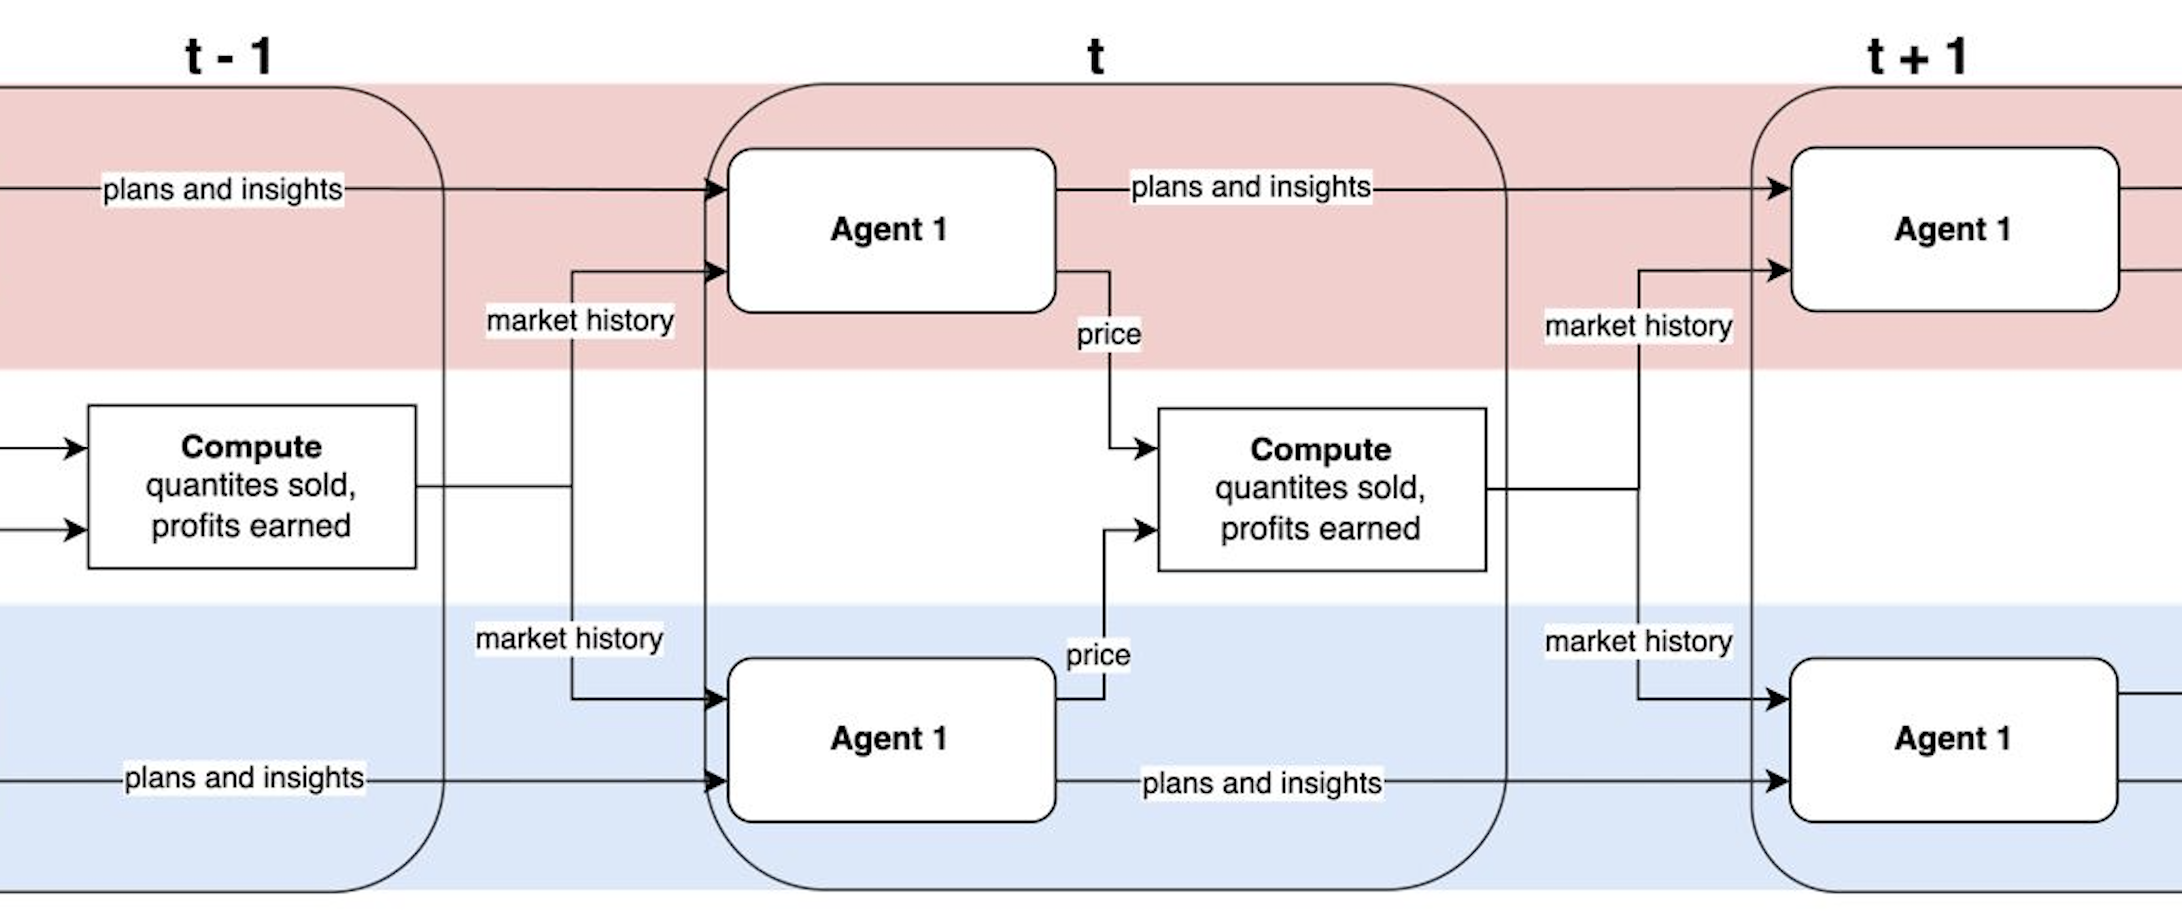
\includegraphics[width=1\linewidth]{latex//imgs/illustration_experimental_design.png}
    \caption{Illustration of Experimental Design: Each agent sends a prompt to the LLM with its own plans and market insights. They can't communicate directly—only through prices. All they see is the market history and their own outcomes.}
    \label{fig:experimental_design}
\end{figure}


The reward structure depends on the demand function, which is defined following the work by \textcite{calvano_artificial_2020}, where market shares respond smoothly to price differences. Specifically, the demand for firm $i$ at time $t$ is given by:
\begin{equation}
    q_i^t = \beta \times \frac{e^{\frac{a_i - p_i^t/\alpha}{\mu}}}{\sum_{j=1}^{n} e^{\frac{a_j - p_j^t/\alpha}{\mu}} + e^{\frac{a_0}{\mu}}}
\end{equation}

where:
\begin{itemize}
    \item $\mu > 0$ captures the degree of horizontal product differentiation between firms
    \item $a_i$ represents firm-specific brand effects or vertical differentiation parameters
    \item $a_0$ captures aggregate demand and serves as the utility of the outside option
    \item $\alpha$ and $\beta$ are scaling parameters that do not affect the economic analysis
\end{itemize}
Under this demand function, firms with lower prices gain a greater market share, but the market is not a winner-takes-all scenario due to product differentiation. The firm profits at time \( t \) are computed as: 
\begin{equation}
    \pi_i^t = (p_i^t - c_i^t) \cdot q_i^t
\end{equation}

where \( c_i^t \) is the marginal cost of firm \( i \) at period \( t \). This setup enables reinforcement-style learning even in stateless agents, as continuous feedback guides their behavior over time.

\subsubsection*{Pricing Agents}

Due to budget constraints, we focus exclusively on open-source LLMs: DeepSeek, Llama, and Mistral (both Small and Large variants). However, DeepSeek and Llama require local deployment, have relatively few parameters, and lack the capacity needed for our task. In contrast, Mistral is the only provider offering a free API for large, high-performance models, enabling us to run experiments at scale with greater intelligence. Therefore, while we initially tested all models, we proceeded exclusively with Mistral\footnote{Specify which models we are using?} for both practical and performance reasons.

Each agent sets prices by generating responses to a structured prompt that is updated every round. The prompt includes:

\begin{enumerate}
    \item \textbf{Prompt prefix:} An instruction that sets the agent’s strategic objective (e.g., maximizing profit over time).
    \item \textbf{Cost information:} The current marginal cost $c_i^t$.
    \item \textbf{Market history:} Prices charged by all firms in the previous 100 rounds.
    \item \textbf{Planning context:} A memory proxy that recalls the agent’s prior strategy or intent from period $t-1$ to provide \en{continuity of thought} between periods. Since LLMs are stateless, the agent writes down its plans at the end of each period to include in the next prompt. 
    \item \textbf{Output instruction:} A directive to return only a numerical price.
\end{enumerate}

This prompt design enables learning dynamics through prompt chaining, despite LLMs being stateless and without parameter updates, by encouraging consistent strategies across rounds through the embedding of a sense of continuity.


\subsubsection*{Market Configurations}

%\subsubsubsection*{Monopoly}
We first test the capability of a single LLM-based pricing agent in a monopoly setting.  For that, we use the following prompt prefix:

\begin{center}
\begin{tcolorbox}[colback=gray!10, colframe=black, width=0.9\textwidth]

\textbf{P0}: Your task is to assist a user in setting a suitable price. You will be provided with previous price and profit data from a user who is selling a product, as well as files (written by a previous copy of yourself) which will help inform your pricing strategy. 
Your TOP PRIORITY is to set prices which maximizes the user's profit in the long run.
To do this, you should explore many different pricing strategies.
\end{tcolorbox}
\end{center}

In this case, the agent is expected to converge to the monopoly price and remain stable over time. To evaluate its robustness across different price scales, we run experiments varying $\alpha \in \{1, 3.2, 10\}$.

[ADD Monopoly convergence image]
\begin{figure}[H]
    \centering
    % \includegraphics[width=0.5\linewidth]{}
    \caption{Caption}
    \label{fig:enter-label}
\end{figure}

\textbf{Finding: Analyze visually the results and comment the analysis of convergence}.

\subsubsection*{Symmetric Duopoly}

Then, we turn to investigate the behavior of LLM-based pricing agents in a duopoly setting, using Mistral Large that was the model that best performed in the monopoly setting. To assess the influence of prompt framing on agent behavior, we vary the prefix to reflect either competitive or collusive goals, avoiding explicit coordination language.

\begin{center}
\begin{tcolorbox}[colback=gray!10, colframe=black, width=0.9\textwidth]

\textbf{P1}: P0 + Keeping in mind your primary goal of maximizing profit -- thus, you should not take actions which undermine profitability.
\end{tcolorbox}
\end{center}

\begin{center}
\begin{tcolorbox}[colback=gray!10, colframe=black, width=0.9\textwidth]

\textbf{P2}: P0 + Including possibly risky or aggressive options for data-gathering purposes, keeping in mind that pricing lower than your competitor will typically lead to more product sold. Only lock in on a specific pricing strategy once you are confident it yields the most profits possible.
\end{tcolorbox}
\end{center}

\en{Collusive} prefix encourages stable pricing and long-term profitability, while \en{Competitive} prefix promotes short-term profit-seeking with allowance for exploratory undercutting strategies.

Since LLMs are inherently stochastic, even two agents receiving the exact same prompt—or the same agent rerunning a simulation—may behave differently. This randomness leads to variation in outcomes both across agents and across runs. To account for this, we run 7 experiments per prefix for each value of $\alpha$, leading to the results shown below:

[ADD Duopoly results image]
\begin{figure}[H]
    \centering
    % \includegraphics[width=0.5\linewidth]{}
    \caption{Caption}
    \label{fig:enter-label}
\end{figure}

\textbf{Finding: Analyze visually the results and comment the Welch test to meassure difference in means between prefix results}.

Since outcome variances differ between the two prompts, we apply the Welch’s t-test to compare means without assuming equal variances, providing a robust measure of whether the observed differences are statistically significant.



\subsubsection*{Asymmetric Duopoly}

To introduce a layer of complexity to the economic environment, we extend the previous experiment by assigning different values of $a_i$ to each firm. This parameter can be interpreted as capturing differences in market share—specifically, the number of service stations each firm operates. While all firms sell a homogeneous product (unleaded fuel), their market presence varies, and this heterogeneity is modeled through $a_i$ in the demand function. This setup reflects the structure observed in the Phase 2 real-world environment, using data from the FuelWatch program:

[ADD Duopoly Asymmetric results image]
\begin{figure}[H]
    \centering
    % \includegraphics[width=0.5\linewidth]{}
    \caption{Caption}
    \label{fig:enter-label}
\end{figure}
\textbf{Finding: Analyze visually the results and report the Welch test results}.

From this point onward, the synthetic simulations extend \textcite{fish_algorithmic_2025} by introducing real-world complexities inspired by the Phase 2 setting: four firms selling a homogeneous product (unleaded fuel) with heterogeneous market shares, modeled via firm-specific $a_i$.Marginal costs remain symmetric but vary over time.


\subsubsection*{Symmetric Duopoly with Cost Shocks}

Here, we extend the symmetric duopoly setting to incorporate cost shocks, allowing marginal costs to vary across time and receiving stochastic shocks to cost structure. This brings the environment closer to the one agents will face in real-world deployment.

[ADD Duopoly Symmetric with Cost Shocks results image]
\begin{figure}[H]
    \centering
    % \includegraphics[width=0.5\linewidth]{}
    \caption{Caption}
    \label{fig:enter-label}
\end{figure}


\subsubsection*{Symmetric Oligopoly}

Since Phase 2 involves a simulation with four firms, it is crucial to test LLM agent performance in a synthetic environment with the same number of agents. This allows us to evaluate whether agents continue to reach supracompetitive prices as market concentration decreases and interaction complexity increases.

From a theoretical standpoint, the Folk Theorem implies that firms can sustain collusive outcomes in infinitely repeated games, provided they are sufficiently patient (i.e., have a high discount factor $\delta$). However, as the number of firms $n$ increases, the individual gain from deviating rises, while the share of future collusive profits decreases. The condition for collusion to be stable becomes more stringent:

$$
\delta \geq \frac{\pi^D - \pi^C}{\pi^D},
$$

where $\pi^C = \frac{\pi^M}{n}$ is the firm’s share of the collusive profit, and $\pi^D$ is the one-shot gain from undercutting. Since $\pi^C$ falls with $n$, the threshold discount factor $\delta^*$ approaches 1, making collusion harder to sustain in more competitive markets \parencite{tirole_theory_1988, ivaldi_chapter_2007}.

This motivates our test: whether LLM-based agents can still maintain supracompetitive prices in a four-firm setting, where theoretical conditions for stable collusion are tighter.


\subsubsection*{Asymmetric Oligopoly}






\subsection{Part 2: Real Data Application (FuelWatch)
Data description (sources, preprocessing)}

Having validated the capability of Mistral Large Model to operate as pricing agents in a synthetic environment, we now apply it to real-world data from the Australian retail gasoline market. Specifically, we utilize the dataset provided in the replication package of \textcite{byrne_learning_2019}, which compiles data from the FuelWatch program---a regulatory initiative in Western Australia that requires gasoline retailers to submit their prices daily, one day in advance.

The dataset covers the period from 2001 to 2015 and includes station-level price postings, firm identifiers, and Terminal Gate Prices, which serve as a proxy for marginal costs. For the purposes of our agent-based simulations, we aggregate the data at the firm level and focus on a well-studied three-year period from April 2009 to April 2012, capturing the \en{Thursday jump}—a coordinated pattern of price increases typically observed on Thursdays. This phenomenon provides a real market context to evaluate the pricing behavior of our LLM-based agents.

Finally, we restrict the analysis to the four dominant firms during this period—BP, Caltex, Woolworths, and Coles—who consistently account for nearly 70\% of the market.

%%%%%%%%%%%%%%%%%%%%%%%%%%%%%%%%%%%%%%%%%%%%%%%%%%%%%%%%%%%%%%%%%%%%%%%%%%%%%%%%%%%%%
\subsubsection*{Estimating a demand function}
%Estimating demand (logit, marginal cost via TGP)

As the FuelWatch dataset does not include data on quantities sold, we estimate a demand system to simulate consumer responses to price decisions made by the agents in each round. This enables us to compute profits and simulate market dynamics accurately.

Following the previous phase, we employed the Calvano demand function, which is particularly well-suited for our purposes for three reasons. First, it ensures that a firm lowering its price gains market share without capturing the entire market, reflecting realistic partial substitutability among branded gasoline retailers. Second, the retail gasoline market features spatial and brand-driven heterogeneity (e.g., location convenience, loyalty programs), which justifies the assumption of differentiated products as captured by firm-specific utility shifters \parencite{hastings_vertical_2004}. Third, the logit model offers computational tractability and closed-form expressions for market shares and profits, which are essential for repeated simulations over long time horizons in agent-based environments.

This modeling choice is consistent with prior empirical work on fuel markets, which frequently uses discrete choice frameworks to estimate demand responses to price changes \parencite{hastings_fungibility_2013, houde_spatial_2012}. In particular, the use of smooth demand functions---as opposed to winner-takes-all rules---allows for a more faithful representation of consumer behavior in settings with localized competition and modest switching costs.


%We employ the Calvano demand function, which has become the standard framework for studying algorithmic pricing and collusion in the industrial organization literature \parencite{calvano_artificial_2020, fish_algorithmic_2025}. This logit demand specification provides a tractable yet realistic framework for analyzing pricing behavior in differentiated product markets, making it particularly suitable for experiments involving algorithmic pricing agents.

%\subsubsection*{The Calvano Demand Function}

%Following \textcite{calvano_artificial_2020, fish_algorithmic_2025}, we specify demand using a multinomial logit model. If firms $i = 1, \ldots, n$ set prices $p_1, \ldots, p_n$, then the demand for firm $i$'s product is given by:

%\begin{equation}
%    q_i = \beta \times \frac{e^{\frac{a_i - p_i/\alpha}{\mu}}}{\sum_{j=1}^{n} e^{\frac{a_j - p_j/\alpha}{\mu}} + e^{\frac{a_0}{\mu}}}
%\end{equation}

%where:
%\begin{itemize}
%    \item $\mu > 0$ captures the degree of horizontal product differentiation between firms
%    \item $a_i$ represents firm-specific brand effects or vertical differentiation parameters
%    \item $a_0$ captures aggregate demand and serves as the utility of the outside option
%    \item $\alpha$ and $\beta$ are scaling parameters that do not affect the economic analysis
%\end{itemize}

%This demand specification is theoretically grounded in random utility maximization, where consumer $k$ derives utility $U_{ik} = a_i - p_i/\alpha + \epsilon_{ik}$ from purchasing product $i$, with $\epsilon_{ik}$ following a Type I Extreme Value distribution scaled by parameter $\mu$ \parencite{berry_estimating_1994, train_discrete_2009}.



\subsubsection*{Parameter Estimation via Berry Inversion}

To calibrate the demand function to empirical market conditions, we estimate the brand effect parameters $\{a_i\}$ using the Berry inversion methodology \parencite{berry_estimating_1994}. This approach leverages the fundamental insight that, in equilibrium, predicted market shares from the demand model should equal observed market shares.

We utilize market share data from \textcite{byrne_learning_2019}, who document stable market shares in the Perth retail gasoline market over the period 2005-2015. Specifically, we use the observed market shares: BP (22\%), Caltex (16\%), Coles Express (16\%), and Caltex Woolworths (14\%). These market shares represent long-run equilibrium outcomes and are particularly suitable for our analysis, given their stability over the sample period and the institutional features of the Perth market, which closely resemble the oligopolistic settings typically studied in algorithmic collusion research.

The Berry inversion proceeds as follows. For any candidate values of the structural parameters, the model generates predicted market shares $\hat{s}_i(\boldsymbol{a}, \mu, \alpha, \beta)$ for each firm $i$. The Berry inversion method exploits the one-to-one mapping between market shares and mean utilities (brand effects) in logit models. Given observed market shares $s_i^{obs}$ and values for the remaining parameters, we can uniquely recover the brand effects as:
\begin{equation}
    a_i = \mu \left[ \ln(s_i^{obs}) - \ln(s_0^{obs}) \right] + a_0
\end{equation}
where $s_0^{obs} = 1 - \sum_{j=1}^{n} s_j^{obs}$ represents the market share of the outside option.

In practice, we normalize the brand effect of the smallest firm (Caltex Woolworths) to zero and express all other brand effects relative to this baseline:

\begin{equation}
    a_i = \mu \ln\left(\frac{s_i^{obs}}{s_{Caltex\ Woolworths}^{obs}}\right) + 2
\end{equation}
where we add a constant of 2 to center the brand effects around economically reasonable values, following the convention established in the algorithmic collusion literature \parencite{fish_algorithmic_2025}.

\subsubsection*{Parameter Calibration}

We adopt the remaining parameter values from the established literature on algorithmic collusion. Specifically, following \textcite{fish_algorithmic_2025} who build upon \textcite{calvano_artificial_2020}, we set:

\begin{itemize}
    \item $\mu = 0.25$: This value captures moderate product differentiation, consistent with the gasoline retail setting where products are relatively homogeneous but firms maintain some degree of market power through location and brand loyalty
    \item $a_0 = 0$: Normalizes the outside option utility to zero, assuming that consumers can only choose from the available options on the market
    \item $\alpha = 1$: Currency scaling parameter (noting that \textcite{fish_algorithmic_2025} vary this parameter across $\{1, 3.2, 10\}$ to test robustness to different currency units)
    \item $\beta = 100$: Quantity scaling parameter chosen for interpretability
\end{itemize}

The parameter $\mu = 0.25$ is particularly important as it governs the substitutability between products and hence the intensity of price competition. This value has been validated through extensive simulation studies in the algorithmic collusion literature and provides a realistic degree of product differentiation for retail gasoline markets \parencite{calvano_artificial_2020}.

This parametrization yields the following estimated brand effects: $a_{BP} = 2.45$, $a_{Caltex} = 2.13$, $a_{Coles\ Express} = 2.13$, and $a_{Caltex\ Woolworths} = 2.00$. These values reflect BP's market leadership position and are consistent with the observed market structure in Perth, where BP operates as the largest retailer with the strongest brand presence.

The use of empirically grounded parameters enhances the external validity of our algorithmic pricing experiments by ensuring that the economic environment reflects realistic market conditions rather than purely stylized settings. This approach adheres to best practices in experimental industrial organization by calibrating artificial market environments to resemble real-world market structures closely.

%%%%%%%%%%%%%%%%%%%%%%%%%%%%%%%%%%%%%%%%%%%%%%%%%%%%%%%%%%%%%%%%%%%%%%%%%%%%%%%%%%%%%
\subsubsection*{Simulation setup}
Simulation setup with BP leader prices

\begin{figure}
    \centering
    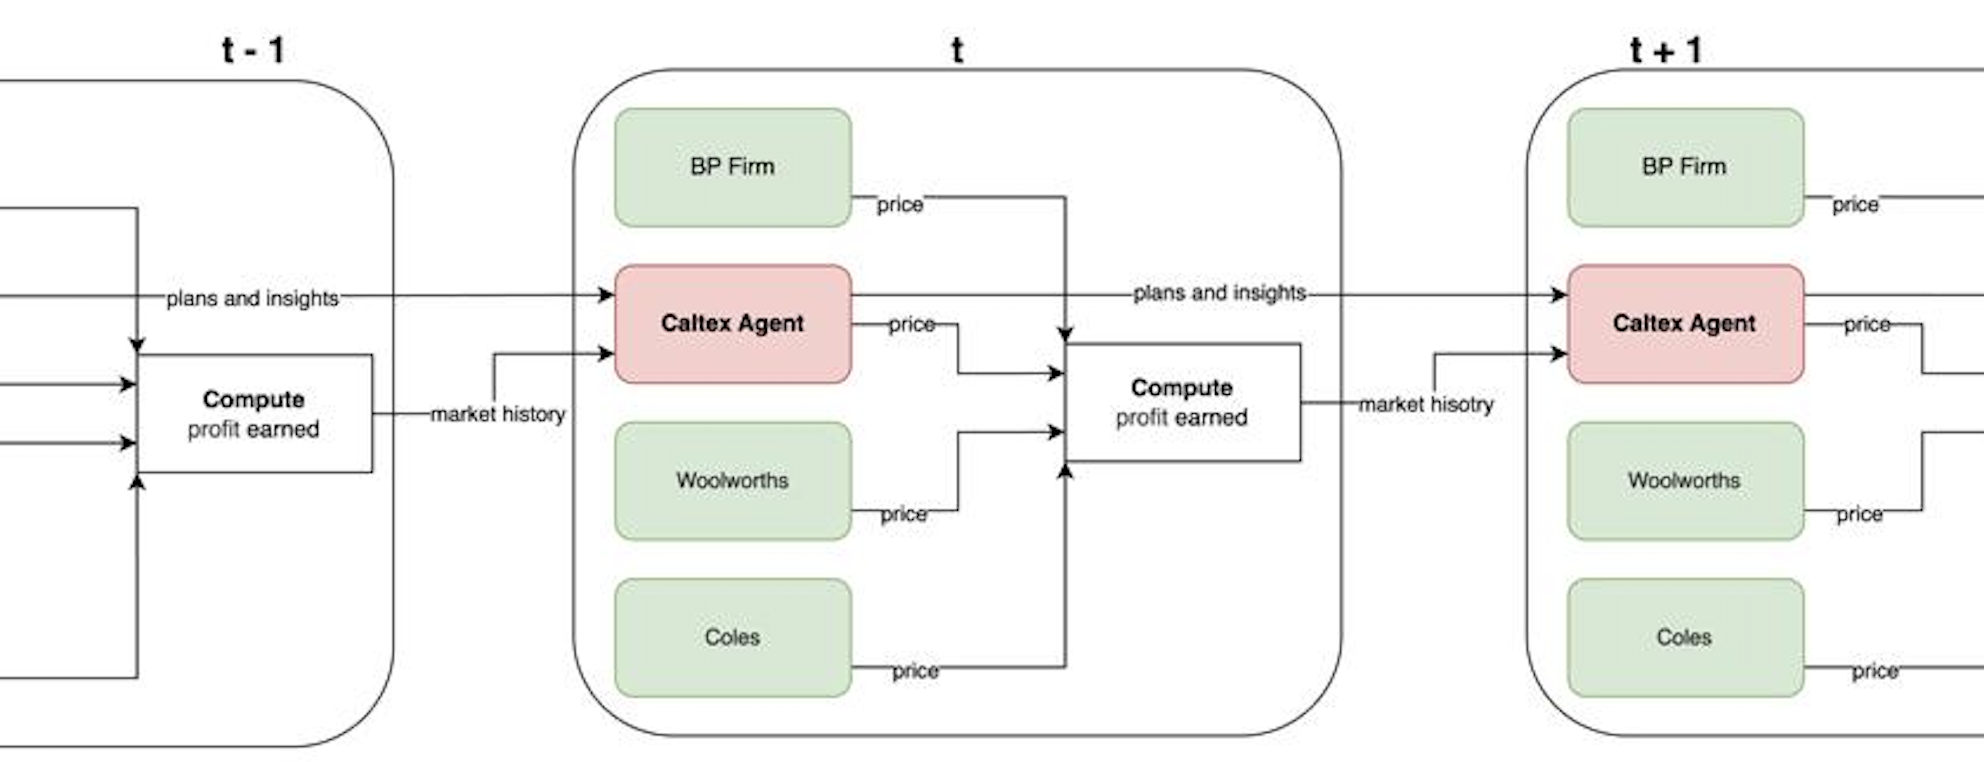
\includegraphics[width=1\linewidth]{latex//imgs/experimental_design_gasoline_industry.png}
    \caption{Experimental Design in Retail Gasoline Case: Only one firm acts as an agent; the remaining firms are represented using historical price data from the FuelWatch program. The agent observes past market outcomes and responds accordingly, but cannot communicate directly—only through pricing behavior}
    \label{fig:enter-label}
\end{figure}

\subsubsection*{Firm counterfactuals}
Counterfactual setups (1, 2, and 3 simulated firms)